 \item Wyświetlanie listy części - scenariusz główny \\
 
 Opis słowny - jest to podstawowy przypadek użycia jeśli chodzi o zarządzanie częściami, gdyż zapewnia on funkcjonalność prezentacji wszystkich dostępnych w sklepie części. Jest to funkcjonalność używana zarówno przez klientów sklepu (w celu przeglądania asortymentu sklepu), jak i przez pracowników (w celu zarządzania częściami). W przypadku gdy użytkownik posiada odpowiednie uprawnienia (pracownik magazynu), lista części udostępnia także funkcjonalności zarządzania częściami (modyfikacja, usuwanie, itd. - dokładnie opisane poniżej).
 
 \begin{longtable}{|p{5cm}|p{7cm}|}
 	\hline
	\textbf{Aktor} & Klient lub pracownik \\
	\hline
	\textbf{Warunki początkowe} & Brak \\
	\hline
	\textbf{Opis przebiegu interakcji} & Wybór prezentacji listy części na stronie głównej sklepu \\
	\hline
	\textbf{Sytuacje wyjątkowe} & Ustawienie kryteriów filtrowania, posiadanie przez użytkownika specjalnych uprawnień do zarządania częściami \\
	\hline
	\textbf{Warunki końcowe} & Wyświetlenie listy dostępnych części \\
	\hline
 \end{longtable}
 
  \item Wyświetlanie listy części - scenariusz główny \label{lista-czesci} \\
  \begin{tabularx}{\linewidth}{ c X}
  Aktor: & Klient lub pracownik \\
  \end{tabularx}
   \begin{enumerate}
    \item Użytkownik (nie posiadający specjalnych uprawnień) uruchamia stronę internetową sklepu i wybiera opcję wyświetlenia listy części.
    \item System prezentuje listę dostępnych dla użytkownika części (możliwych do kupienia), posortowaną alfabetycznie, z podziałem wyników na strony (10 wartości na stronie, z możliwością zmiany tej liczby przez użytkownika na 25, 50 i 100).
  \end{enumerate}
  
  \item Wyświetlanie listy części - scenariusz alternatywny - ustawiono kryteria filtrowania \\
  \begin{tabularx}{\linewidth}{ c X}
  Aktor: & Klient lub pracownik \\
  \end{tabularx}
   \begin{enumerate}
     \item Krok 1 scenariusza głównego.
     \item Użytkownik ustawia żądane przez siebie kryteria filtrowania. Filtrować można po kodzie części, jej nazwie, opisie i cenie.
     \item System prezentuje odfiltrowaną listę części. Sposób prezentacji taki sam jak w scenariuszu głównym, kroku 2.
   \end{enumerate} 
   
   \item Wyświetlanie listy części - scenariusz alternatywny - użytkownik posiada specjalne uprawnienia do zarządzania częściami \\
   \begin{tabularx}{\linewidth}{ c X}
	Aktor: & Pracownik \\
  	\end{tabularx}   
  	\begin{enumerate}
     \item Krok 1 scenariusza głównego.
  	  \item System prezentuje listę części w taki sam sposób jak dla kroku 2 scenariusza głównego, ale dodatkowo przy każdym elemencie listy dostępne są przyciski, umożliwiające pracownikowi edycję danych części lub usunięcie jej z systemu. Na tym ekranie widoczny jest także przycisk umożliwiający dodanie nowego typu części do systemu. Działanie tych przycisków opisane jest w kolejnych przypadkach użycia. Dodatkowo na liście widoczne są także części ukryte (niewidoczne dla kupujących).
  	\end{enumerate}	
  	
\begin{figure}[h!]
    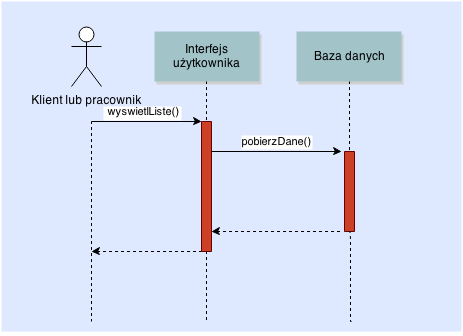
\includegraphics[width=\textwidth,
    height=0.5\textheight]{graphics/UseCase/Czesci/ListaCzesciSD.png}
  \caption{Diagram sekwencji dla przypadku użycia Lista części - scenariusz główny}
\end{figure}